\pdfminorversion=7
\documentclass[11pt]{article}
\usepackage[T1]{fontenc}
\usepackage{lmodern}
\usepackage[margin=1in]{geometry}
\usepackage{amsmath,amssymb,amsthm,mathtools}
\usepackage{microtype}
\usepackage{enumitem}
\usepackage{xcolor}
\usepackage{tikz}
\usetikzlibrary{arrows.meta,positioning}
\definecolor{linkblue}{RGB}{26,65,110}
\PassOptionsToPackage{hyphens}{url}
\usepackage[colorlinks=true,linkcolor=linkblue,citecolor=linkblue,urlcolor=linkblue]{hyperref}
\hypersetup{pdftitle={The Artinian Lex-Plus-Powers Betti Theorem},pdfauthor={OpenAI}}
\pdfinfoomitdate=1
\pdftrailerid{}
\pdfsuppressptexinfo=15
\setlength{\emergencystretch}{2em}
\setlist{itemsep=3pt,topsep=5pt}
\newtheorem{theorem}{Theorem}[section]
\newtheorem{proposition}[theorem]{Proposition}
\newtheorem{lemma}[theorem]{Lemma}
\newtheorem{corollary}[theorem]{Corollary}
\theoremstyle{definition}
\newtheorem{definition}[theorem]{Definition}
\theoremstyle{remark}
\newtheorem{remark}[theorem]{Remark}
\numberwithin{equation}{section}
\newcommand{\C}{\mathbb C}
\newcommand{\N}{\mathbb Z_{\ge0}}
\newcommand{\Z}{\mathbb Z}
\newcommand{\Q}{\mathbb Q}
\DeclareMathOperator{\Tor}{Tor}
\DeclareMathOperator{\Hilb}{Hilb}
\DeclareMathOperator{\Lex}{Lex}
\DeclareMathOperator{\rank}{rank}
\DeclareMathOperator{\Sym}{Sym}
\DeclareMathOperator{\inm}{in}
\title{The Artinian Lex-Plus-Powers Betti Theorem}
\author{OpenAI}
\date{September 23, 2026}
\begin{document}
\maketitle
\begin{abstract}
We prove the Eisenbud--Green--Harris and lex-plus-powers conjectures over every
characteristic-zero field for homogeneous regular sequences of any positive
length, with degrees at least two. For every homogeneous ideal containing such
a sequence, the corresponding lex-plus-powers ideal has the same Hilbert
function and at least as large a graded Betti number in every homological and
internal degree.
\end{abstract}
\tableofcontents
\section{Introduction}\label{sec:introduction}

A Hilbert function records the dimensions of a graded quotient; its graded
Betti numbers also record the relations among its generators and all higher
syzygies. The lex-plus-powers conjecture predicts one extremal ideal for
both kinds of data when the original ideal contains a regular sequence.
We prove its full Artinian form over \(\C\), and deduce the full
characteristic-zero statement for regular sequences of arbitrary positive
length by the established Artinian reduction and coefficient-field descent.

Let
\[
 S=\C[x_1,\ldots,x_n],\qquad
 2\le a_1\le\cdots\le a_n,\qquad
 P=(x_1^{a_1},\ldots,x_n^{a_n}),
\]
where each variable has degree one. Lexicographic order always has
\(x_1>\cdots>x_n\), and a lex segment starts with the \emph{greatest}
monomials. Suppose that a homogeneous ideal \(I\subseteq S\) contains a
homogeneous regular sequence \(f_1,\ldots,f_n\) with \(\deg f_i=a_i\).
Here regularity means that multiplication by \(f_i\) is injective on
\(S/(f_1,\ldots,f_{i-1})\) for each \(i\). Its full length makes
\(S/I\) Artinian: the complete-intersection Hilbert series is
\(\prod_i(1+z+\cdots+z^{a_i-1})\).
For each \(d\ge0\), prescribe
\begin{equation}
 J_d=L_d+P_d,\qquad \dim_\C J_d=\dim_\C I_d,
 \label{eq:prescription}
\end{equation}
where \(L_d\) is the largest lex-segment subspace with this property.
Part of the assertion below is that these dimensions can be attained
and that the prescribed spaces form an ideal.

For a standard graded polynomial ring \(A\) over a field \(F\), write
\[
 \beta^A_{p,j}(B)=\dim_F\Tor^A_p(B,F)_j,
 \qquad F=A/A_{>0}.
\]
The index \(p\) is the homological degree and \(j\) is the internal degree.

\begin{theorem}\label{thm:main}
For every \(n\ge1\), every ordered degree sequence
\(2\le a_1\le\cdots\le a_n\), and every homogeneous ideal
\(I\subseteq\C[x_1,\ldots,x_n]\) containing a regular sequence of these
degrees, the spaces in \eqref{eq:prescription} exist and
\(J=\bigoplus_{d\ge0}J_d\) is a homogeneous ideal. For this single ideal,
\[
 \beta^S_{p,j}(S/I)\le\beta^S_{p,j}(S/J)
 \qquad\text{for every \(p\ge0\) and \(j\in\Z\)}.
\]
There is no restriction on the degrees or number of the additional
generators of \(I\).
\end{theorem}

Thus Theorem~\ref{thm:main} resolves the Artinian lex-plus-powers
conjecture positively over \(\C\).
Its Hilbert-function assertion is the Artinian Eisenbud--Green--Harris
statement; the Betti inequalities are stronger.

The Artinian restriction can be removed from these two conclusions.
Caviglia and Maclagan proved the Artinian reduction for the
Eisenbud--Green--Harris conjecture \cite[Proposition~10]{CM08};
Caviglia and Kummini proved the corresponding reduction for
lex-plus-powers Betti numbers \cite[Section~4, Theorem~4.1]{CK14}.
Together with a finite coefficient-field descent, these reductions give
the following form over every characteristic-zero field.

\begin{corollary}[Eisenbud--Green--Harris and lex-plus-powers in characteristic zero]
\label{cor:characteristic-zero}
Let \(F\) be a field of characteristic zero, let
\[
 S_F=F[x_1,\ldots,x_n],\qquad
 1\le c\le n,\qquad 2\le a_1\le\cdots\le a_c,
 \qquad P_F=(x_1^{a_1},\ldots,x_c^{a_c}),
\]
with the standard grading and lexicographic order \(x_1>\cdots>x_n\).
Suppose that a homogeneous ideal \(I\subseteq S_F\) contains a homogeneous
regular sequence \(f_1,\ldots,f_c\) with \(\deg f_i=a_i\).
For \(d\ge0\), put
\[
 q_d=\dim_F I_d-\dim_F(P_F)_d.
\]
This integer lies between zero and the number of degree-\(d\) monomials
outside \(P_F\). Let \(J_d\) be the sum of \((P_F)_d\) and the span of the
\(q_d\) lexicographically greatest such monomials. Then
\(J=\bigoplus_{d\ge0}J_d\) is a homogeneous ideal, and for this single ideal
\[
 \dim_F(S_F/I)_d=\dim_F(S_F/J)_d\quad(d\ge0),\qquad
 \beta^{S_F}_{p,j}(S_F/I)\le\beta^{S_F}_{p,j}(S_F/J)
 \quad(p\ge0,\ j\in\Z).
\]
There is no restriction on the degrees or number of the additional
generators of \(I\).
\end{corollary}

Corollary~\ref{cor:characteristic-zero} includes non-Artinian quotients
and fields that are not algebraically closed. The case with no prescribed
regular sequence is the classical lex-ideal theorem cited below.
The division-coefficient construction itself remains the full-length
construction over \(\C\); Section~\ref{sec:characteristic-zero} proves
the corollary from Theorem~\ref{thm:main}.

\subsection{Context and previous results}

The Eisenbud--Green--Harris (EGH) Hilbert-function conjecture arose in
their work on higher Castelnuovo theory \cite[Section~4]{EGH}.
The lex-plus-powers conjecture, generally attributed to Charalambous
and Evans, strengthens that prediction to graded Betti numbers.
Francisco and Richert discuss its origins and identify its first
printed appearance in the work of Evans and Richert
\cite[Section~5]{FR}; see also the public formulations in
\cite[Section~1]{Richert} and
\cite[Conjectures~1.1 and 1.2]{CS}.
Without a prescribed regular sequence, the extremality of lex ideals
at fixed Hilbert function is the theorem of Bigatti, Hulett, and
Pardue \cite{Bigatti,Hulett,Pardue}.
The additional powers encode the degrees of the regular sequence and
give the sharper comparison studied here.
For ideals already containing these powers, Clements--Lindstr\"om
compression supplies the Hilbert-function comparison \cite{CL}.

The prescribed-powers Betti comparison developed through several stages.
Mermin, Peeva, and Stillman proved the comparison for ideals containing
the squares of the variables in characteristic zero
\cite[Theorem~1.1]{MPS}; Murai established it for strongly stable ideals
plus the prescribed powers over any field \cite[Theorem~1.1]{Murai}.
Mermin and Murai then proved the lex-plus-powers comparison for ideals
containing a monomial regular sequence, again over every field
\cite[Theorems~3.1 and 8.1]{MM}. They also isolated the reduction to a
Hilbert-matching monomial ideal with no smaller graded Betti numbers
\cite[Conjecture~10.2]{MM}. It is this reduction that we obtain from
division coefficients. Our proof of the subsequent monomial comparison
is included for completeness; its conclusion is not new.

For nonmonomial regular sequences, the Hilbert-function and Betti problems
have had different ranges of known cases. Abedelfatah proved EGH for full
regular sequences whose forms split into linear factors
\cite[Corollary~4.3]{Abedelfatah15}. Caviglia and Maclagan established
EGH for fast-growing degrees \cite{CM08}, and Caviglia and De Stefani
weakened the required growth to
\(a_i\ge\sum_{j<i}(a_j-1)\) for \(i\ge3\)
\cite[Theorem~A]{CDeS20}. These Hilbert-function results hold over any
field. The characteristic-zero Betti theorem of Caviglia and Sammartano
requires
\(a_i\ge1+\sum_{j<i}(a_j-1)\) for \(i\ge3\)
\cite[Theorem~3.8]{CS}. No such growth condition is imposed here.

More recently, Kuzmanovski \cite[Theorem~1.9]{Kuzmanovski} obtained
asymptotic Betti estimates in characteristic zero in a bounded degree range,
for fixed regular-sequence degree offsets and generator counts and
sufficiently large initial degree. That comparison uses the
reverse-lexicographic generic initial ideal of a lex-plus-powers ideal,
rather than the lex-plus-powers ideal itself as in Theorem~\ref{thm:main}.

Our treatment of the monomial comparison retains the
resolution-level mechanism of distractions
\cite[Theorem~2.19 and Corollary~2.20]{BCR} and the endpoint
decomposition for stable-plus-powers ideals
\cite[Lemma~3.7]{CS}, while organizing the last comparison through ranks
in the Koszul complex.

\subsection{The reduction that carries the Betti numbers}

The essential step is to find a monomial ideal \(M\supseteq P\) such that
\begin{equation}\label{eq:overview-bound}
 \Hilb(S/I)=\Hilb(S/M),\qquad
 \beta^S_{p,j}(S/I)\le\beta^S_{p,j}(S/M)
 \quad\text{for all \(p,j\)}.
\end{equation}
Matching Hilbert functions alone cannot give the second conclusion.

Theorem~1.1 of the companion article \cite{ArtinianEGH} supplies a field
\(k/\C\), a finite-dimensional central division \(k\)-algebra \(\Delta\), and commuting linear
forms \(t_1,\ldots,t_n\) in \(N=\Delta[x_1,\ldots,x_n]\). They satisfy
triangular power identities adapted to the \(f_i\), and their ordered
monomials form a left-\(\Delta\) basis of \(N\).
Section~\ref{sec:forms} states exactly the input needed here, including
the basis assertion for the full algebra rather than only its
complete-intersection quotient.

Let \(T=k[y_1,\ldots,y_n]\) act on \(N\) on the right by \(y_i\mapsto t_i\).
Then \(N\) is simultaneously left-\(S\) free and right-\(T\) free, the
latter of rank \(m=\dim_k\Delta\), with generators in degree zero.
A minimal \(S\)-resolution of \(S/I\) therefore gives a
\emph{minimal} \(T\)-resolution of \(N/IN\), multiplying every Betti number
by the same factor \(m\). With a monomial order adapted to the triangular
identities, the leading coefficient spaces of \(IN\) in the
\(t^\alpha\)-expansion are left ideals of \(\Delta\), hence either zero
or all of \(\Delta\). Their nonzero positions define \(M\); the
triangular identities ensure that \(M\) contains \(P\). A filtered
Koszul comparison then gives \eqref{eq:overview-bound} after cancelling
\(m\).
This resolution transfer is the additional ingredient beyond the
Hilbert-function reduction in \cite{ArtinianEGH}.

Starting from \(M\), we work with the monomials in the exponent box
\(0\le u_i<a_i\). A transfer replaces a factor \(x_\ell\) by \(x_h\),
where \(h<\ell\), provided the result remains in the box.
Root-of-unity distractions followed by initial ideals produce an ideal
\(H\supseteq P\) closed under these transfers, with unchanged Hilbert
function and no smaller quotient Betti numbers. In each degree, replace
the box monomials belonging to \(H\) by the same number of greatest
lexicographic monomials in the box, and retain \(P\). Comparing their bounded
shadows---the multiples by one variable that remain in the box---shows
that the resulting space \(G\) is an ideal.

For the Betti comparison, put \(z=x_n\). The modules \(H/zH\) and
\(G/zG\) over the earlier variables have equal Hilbert functions and
retain the Betti numbers of the ideals \(H\) and \(G\). They split
into components according to the exponent of \(z\), from \(0\) to
\(a_n\). Stability makes every earlier variable annihilate the
components at exponents \(1,\ldots,a_n-1\). Only the two extreme
components can therefore contribute nonzero ranks to the Koszul
differentials. The comparisons on the box slices \(u_n=0\) and
\(u_n=a_n-1\), induction in the number of variables, and monotonicity
of differential ranks under submodules and quotients compare these
endpoint contributions. Since the Koszul terms have equal dimensions,
the resulting reverse inequality for adjacent rank sums gives the
required Betti bound.

Sections~\ref{sec:filtered} and \ref{sec:monomial} establish the filtered
comparison and the transfer to \(M\).
Sections~\ref{sec:stabilization}--\ref{sec:tor} give the complete monomial
comparison. Section~\ref{sec:assembly} identifies its output with
\eqref{eq:prescription} and proves Theorem~\ref{thm:main}.
Section~\ref{sec:characteristic-zero} then removes the Artinian and
complex-coefficient restrictions from the Hilbert and Betti conclusions.

\section{Commuting forms with division coefficients}\label{sec:forms}

We state the construction theorem from the companion article
\cite{ArtinianEGH} in the precise form used below. A central
division algebra over \(k\) is a finite-dimensional
\(k\)-algebra with center \(k\) in which every nonzero element is invertible.
In \(\Delta[x]\), the variables \(x_i\) are central and have degree one,
and elements of \(\Delta\) have degree zero.

\begin{theorem}[Commuting-form construction, {\cite[Theorem~1.1]{ArtinianEGH}}]
\label{thm:forms}
Let \(f_1,\ldots,f_n\) be a homogeneous regular sequence in
\(\C[x_1,\ldots,x_n]\), of degrees \(2\le a_1\le\cdots\le a_n\).
There are a field extension \(k/\C\), a central division \(k\)-algebra
\(\Delta\), and a commutative graded \(k\)-subalgebra
\[
 k[x_1,\ldots,x_n]\subseteq A\subseteq N=\Delta[x_1,\ldots,x_n]
\]
generated by finitely many elements of degree one, containing
\(t_1,\ldots,t_n\in A_1\), such that
\begin{equation}\label{eq:triangular-forms}
 t_h^{a_h}=c_h f_h+\sum_{\ell<h}B_{h\ell}f_\ell
                  +\sum_{\ell>h}C_{h\ell}t_\ell
 \qquad(1\le h\le n).
\end{equation}
Here \(c_h\in k^\times\), \(B_{h\ell},C_{h\ell}\in A\), and every summand
has degree \(a_h\). Moreover,
\[
 \{t^\alpha=t_1^{\alpha_1}\cdots t_n^{\alpha_n}:
       \alpha\in\N^n\}
\]
is a graded left-\(\Delta\) basis of the \emph{full} algebra \(N\).
\end{theorem}

The basis assertion in Theorem~\ref{thm:forms} is stronger than a basis of the finite
complete-intersection quotient: every monomial \(t^\alpha\), without
an upper bound on its exponents, occurs in the decomposition of \(N\).
This is what will make \(N\) a free module over a polynomial ring and
allow us to transfer an entire resolution. The Hilbert-function
consequence of the foundation theorem alone would not suffice.

\begin{remark}\label{rem:coefficients}
Commutativity of the forms does not mean that their individual
\(\Delta\)-coefficients commute. The proof below always places those
coefficients on the left and multiplies by the \(t_i\) on the right.
The construction itself has no hypothesis on the additional generators
of \(I\).
\end{remark}

\section{Graded resolutions and leading coefficient spaces}
\label{sec:filtered}

We first prove a comparison for quotients of a free module whose monomial
positions have vector-space coefficients.  The application in the next
section will use a division algebra as that coefficient space.  The
comparison must retain each internal degree separately, so we work with
the graded Koszul complex throughout.

Let $F$ be a field and let $A=F[y_1,\ldots,y_r]$, with each variable of
degree one.  For a finitely generated graded $A$-module $B$, put
\[
 \beta^A_{p,j}(B)=\dim_F\Tor^A_p(B,F)_j,
 \qquad F=A/(y_1,\ldots,y_r).
\]
We use the shift convention $B(-s)_d=B_{d-s}$.  All modules considered
below are bounded below and have finite-dimensional graded components.

\begin{lemma}[Minimal graded resolutions]
\label{filt:minimal}
Every finitely generated graded $A$-module $B$ has a graded free resolution
whose differentials have entries in $A_{>0}$.  In such a resolution, the
number of free generators of degree $j$ in homological position $p$ is
$\beta^A_{p,j}(B)$.  If $H\subsetneq A$ is a homogeneous ideal, then
\begin{equation}
 \beta^A_{p+1,j}(A/H)=\beta^A_{p,j}(H)
 \qquad(p\geq 0,\ j\in\Z).
 \label{filt:ideal-quotient}
\end{equation}
If $H$ is monomial, a minimal resolution of $A/H$ can be chosen
homogeneous for the exponent multigrading, with all generator
multidegrees in $\Z_{\geq0}^r$.
\end{lemma}

\begin{proof}
Lift a homogeneous $F$-basis of $B/A_{>0}B$ to $B$ and map the free module
on these lifts to $B$.  This map is surjective: in each degree, an element
not yet expressed in the lifts differs from such an expression by a sum
of positive-degree multiples of elements of smaller degree, to which
induction applies.  Its kernel is finitely generated because $A$ is
Noetherian.  Repeating the construction for successive kernels gives a
free resolution.  At each stage, reduction modulo $A_{>0}$ identifies the
chosen free generators with a basis of the corresponding module modulo
$A_{>0}$, so the next kernel lies in $A_{>0}$ times that free module.
Thus every differential between free modules has positive-degree
entries.  Tensoring with $F$ makes these differentials zero and proves
the assertion about $\Tor$.

A minimal resolution of a proper homogeneous ideal $H$, followed by
the inclusion $H\hookrightarrow A$ and the quotient $A\twoheadrightarrow
A/H$, is a minimal resolution of $A/H$: the additional entries also
have positive degree since $H\subseteq A_{>0}$.  This proves
\eqref{filt:ideal-quotient}, including $H=0$.

For a monomial quotient, carry out the same construction with
multihomogeneous lifts.  The initial free module is $A$ in multidegree
zero.  A free module whose generator multidegrees are nonnegative has
no component in a multidegree outside $\Z_{\geq0}^r$; neither does its
kernel or a quotient of that kernel.  Induction therefore gives the
last assertion.
\end{proof}

\begin{lemma}[Koszul calculation]
\label{filt:koszul}
Let $K_\bullet(B)$ be the Koszul complex on $y_1,\ldots,y_r$ with
coefficients in $B$.  Its term of internal degree $j$ in position $p$ is
\[
 K_p(B)_j=\bigoplus_{\substack{\sigma\subseteq\{1,\ldots,r\}\\
                              |\sigma|=p}} B_{j-p}e_\sigma,
\]
where $e_\sigma$ has degree $p$.  Its homology satisfies
\[
 \dim_F H_p(K_\bullet(B)_j)=\beta^A_{p,j}(B).
\]
\end{lemma}

\begin{proof}
For $\sigma=\{i_1<\cdots<i_p\}$ the differential is
\[
 d(be_\sigma)=\sum_{q=1}^p(-1)^{q-1}y_{i_q}b\,
                    e_{\sigma\setminus\{i_q\}}.
\]
The complex $K_\bullet(A)$ is the tensor product over $F$ of the
one-variable complexes
\[
 0\longrightarrow F[y_i](-1)
   \xrightarrow{\ y_i\ }F[y_i]\longrightarrow0.
\]
Each has homology $F$ in position zero and no other homology.  A complex
of vector spaces splits as its homology with zero differential plus
contractible two-term summands.  Tensoring these splittings shows that
$K_\bullet(A)$ is a free resolution of $F$.

To compare this computation with a resolution of $B$, take any graded
free resolution $F_\bullet\to B$ and form the first-quadrant double
complex $F_\bullet\otimes_A K_\bullet(A)$.  Augmenting either factor
gives maps from its total complex to $F_\bullet\otimes_A F$ and to
$B\otimes_A K_\bullet(A)$, respectively.  The kernels have exact columns
or exact rows, since the terms of the other factor are free.  Their
total complexes are exact.  For exact columns, eliminate a cycle's
component of greatest horizontal index by a vertical boundary; the
correction introduces terms only in the next column to the left.
There are finitely many components on each total-degree diagonal,
so iteration eliminates the cycle.  The argument for exact rows
interchanges the two indices.  Both augmentation maps consequently induce
homology isomorphisms.  This identifies the homology of
$B\otimes_A K_\bullet(A)=K_\bullet(B)$ with $\Tor^A(B,F)$, preserving
the internal grading.
\end{proof}

We now order monomial positions without choosing an order on their
coefficients.  Let $V$ be a finite-dimensional $F$-vector space in
degree zero, and set
\[
 E=V\otimes_F A=\bigoplus_{\alpha\in\Z_{\geq0}^r}Vy^\alpha.
\]
Choose a total order $\prec$ on the exponents of each fixed total
degree, compatible with addition: if $\alpha\prec\beta$, then
$\alpha+\gamma\prec\beta+\gamma$ for every
$\gamma\in\Z_{\geq0}^r$.  The first nonzero position of an element is
its leading position in this order.

For a homogeneous submodule $W\subseteq E$ and an exponent $\alpha$,
define
\[
 V_\alpha=\left\{v\in V:
   vy^\alpha+\sum_{\substack{|\gamma|=|\alpha|\\\alpha\prec\gamma}}
        v_\gamma y^\gamma\in W
        \text{ for some }v_\gamma\in V\right\}.
\]
This is an $F$-subspace of $V$.  The resulting leading submodule is
\[
 \operatorname{in}_{\prec}W
       =\bigoplus_{\alpha\in\Z_{\geq0}^r}V_\alpha y^\alpha.
\]
Indeed, multiplication of a witnessing element by $y_i$ shows that
$V_\alpha\subseteq V_{\alpha+e_i}$, so this direct sum is an
$A$-submodule.

\begin{proposition}[Leading-submodule comparison]
\label{filt:comparison}
\label{filt:initial}
With $A,V,E,W$ and $\prec$ as above, for every $d\in\Z$, every
$p\geq0$, and every $j\in\Z$ one has
\begin{align}
 \dim_F(E/W)_d
    &=\dim_F(E/\operatorname{in}_{\prec}W)_d,
       \label{filt:hilbert}\\
 \beta^A_{p,j}(E/W)
    &\leq\beta^A_{p,j}(E/\operatorname{in}_{\prec}W).
       \label{filt:betti}
\end{align}
\end{proposition}

\begin{proof}
Write $Q=E/W$.  In degree $d\geq0$, let $E_{\succeq\alpha}$ be the
sum of the positions $Vy^\gamma$ with $|\gamma|=d$ and
$\alpha\preceq\gamma$, and define $E_{\succ\alpha}$ similarly with
strict inequality.  Their images in $Q_d$ give a finite descending
filtration.  Its quotient at $\alpha$ is
\begin{equation}
 \frac{\operatorname{im}(E_{\succeq\alpha}\to Q_d)}
      {\operatorname{im}(E_{\succ\alpha}\to Q_d)}
 \simeq
 \frac{E_{\succeq\alpha}}
      {E_{\succ\alpha}+(W_d\cap E_{\succeq\alpha})}
 \simeq (V/V_\alpha)y^\alpha.
 \label{filt:slot-quotient}
\end{equation}
The last isomorphism takes the coefficient at $\alpha$.  Summing its
dimensions proves \eqref{filt:hilbert}; both sides vanish for $d<0$.

Fix an internal degree $j\geq0$.  We give all terms of
$K_\bullet(Q)_j$ a common filtration indexed by the degree-$j$
exponents.  For a subset $\sigma$, put
$\mathbf{1}_\sigma=\sum_{i\in\sigma}e_i$.  In the summand with
exterior label $e_\sigma$, place the coefficient position $\alpha$ at
\[
                    \alpha+\mathbf{1}_\sigma.
\]
More explicitly, the filtration subspace at $\beta$ in that summand
is the image of the span of all $Vy^\alpha$ satisfying
$\beta\preceq\alpha+\mathbf{1}_\sigma$.  The full filtration subspace
is the direct sum over the labels $\sigma$.  Addition compatibility
means that the relative order of the positions within one summand
agrees with their order in $Q_{j-|\sigma|}$.

A differential deleting $i\in\sigma$ multiplies its coefficient by
$y_i$.  It sends the position with exponent $\alpha$ to that with
exponent $\alpha+e_i$, and
\[
 (\alpha+e_i)+\mathbf{1}_{\sigma\setminus\{i\}}
       =\alpha+\mathbf{1}_\sigma.
\]
Thus the differential preserves the filtration.  By
\eqref{filt:slot-quotient}, its map on the corresponding associated
graded positions is, up to the Koszul sign,
\[
 V/V_\alpha\longrightarrow V/V_{\alpha+e_i},
 \qquad [v]\longmapsto[v].
\]
This is well defined by $V_\alpha\subseteq V_{\alpha+e_i}$.
Consequently the associated graded complex is exactly
$K_\bullet(E/\operatorname{in}_{\prec}W)_j$, decomposed by the total
exponent $\beta$.

For completeness, if $d:C\to C'$ is a filtration-preserving linear
map between finite-dimensional filtered spaces, the filtration induced
on $\ker d$ gives an injection
\[
          \operatorname{gr}(\ker d)
               \hookrightarrow\ker(\operatorname{gr}d).
\]
Indeed a leading class represented by an element of $\ker d$ maps to
zero, and the induced filtration on the kernel makes this inclusion
injective.  Since taking associated graded preserves dimension, it
follows that
$\operatorname{rank}d\geq\operatorname{rank}(\operatorname{gr}d)$.
At a fixed term of a complex, the homology dimension is the term
dimension minus the ranks of its incoming and outgoing maps.  Applying
the rank inequality to these two maps proves that passing to the
associated graded complex cannot decrease this homology dimension.
Lemma~\ref{filt:koszul} now gives \eqref{filt:betti}.  For $j<0$ all
the relevant Koszul terms vanish, so the same assertion holds.
\end{proof}

Taking $V=F$ recovers the usual comparison with a monomial initial
ideal; see also \cite[Section~2]{MM}. Keeping $V$ arbitrary is essential
for the next application:
the coefficient algebra will enlarge all dimensions by the same
finite factor, which can then be cancelled.

\section{A monomial bound containing the prescribed powers}
\label{sec:monomial}

We use the commuting forms of Theorem~\ref{thm:forms} to construct a
monomial ideal containing the prescribed powers.  The construction
preserves the Hilbert function and increases every graded Betti number.
The first step explains why the original resolution remains minimal
over the polynomial ring acting through these forms.

\begin{lemma}[Transfer of a minimal resolution]
\label{mono:transfer}
Let $S=\C[x_1,\ldots,x_n]$, let $k$ be a field containing $\C$, and
let $\Delta$ be a finite-dimensional central division $k$-algebra.
Put $m=\dim_k\Delta$ and
$N=\Delta[x_1,\ldots,x_n]$, where the $x_i$ are central.
Suppose that $t_1,\ldots,t_n\in N_1$ commute and that
\begin{equation}
          N=\bigoplus_{\alpha\in\Z_{\geq0}^n}\Delta t^\alpha
 \label{mono:basis}
\end{equation}
is a graded direct-sum decomposition.  Give
$T=k[y_1,\ldots,y_n]$ a right action on $N$ by multiplication,
$u\cdot y_i=ut_i$.
For every homogeneous ideal $I\subseteq S$, the right $T$-module
$Q=N/IN$ satisfies
\begin{align}
 \dim_k Q_d&=m\dim_\C(S/I)_d
          &&(d\in\Z),\label{mono:dimension-transfer}\\
 \beta^T_{p,j}(Q)&=m\beta^S_{p,j}(S/I)
          &&(p\geq0,\ j\in\Z).
          \label{mono:betti-transfer}
\end{align}
Here right and left modules over the commutative ring $T$ are
identified when computing $\Tor$.
\end{lemma}

\begin{proof}
Commutativity of the $t_i$ and centrality of $k$ make the stated right
$T$-action well defined.  The map
\begin{equation}
 \Delta\otimes_kT\longrightarrow N,
 \qquad b\otimes y^\alpha\longmapsto bt^\alpha
 \label{mono:free-map}
\end{equation}
is a graded vector-space isomorphism by \eqref{mono:basis}.  It is
right $T$-linear because $(bt^\alpha)t_i=bt^{\alpha+e_i}$.
Thus $N$ is right $T$-free of rank $m$, with a basis in degree zero,
and
\begin{equation}
                         N_{>0}=NT_{>0}.
 \label{mono:positive-degree}
\end{equation}

The left $S$-action commutes with the right $T$-action by associativity
of multiplication in $N$.  Moreover,
$N=\Delta\otimes_\C S$ as a left $S$-module, so $N$ is left $S$-free
and therefore flat.  Each element of $I$ is central in $N$, whence
$IN$ is a two-sided ideal.  In particular it is a right $T$-submodule,
and
\[
               Q\simeq\Delta\otimes_\C(S/I).
\]
Taking a complex basis of $(S/I)_d$ proves
\eqref{mono:dimension-transfer}.

Let $F_\bullet\to S/I$ be a minimal graded $S$-free resolution.
Since $S$ is commutative, regard its terms as right $S$-modules and
tensor with the $(S,T)$-bimodule $N$.  Flatness gives a resolution
\[
                    F_\bullet\otimes_SN\longrightarrow Q
\]
by graded free right $T$-modules.  An entry $f$ of an original
differential acts on $N$ by left multiplication.  This map is right
$T$-linear, again by associativity.

Choose a $k$-basis $b_1,\ldots,b_m$ of $\Delta$, which is a right
$T$-basis of $N$ under \eqref{mono:free-map}.  If $f$ is nonzero and
has degree $e>0$, then each $fb_u$ belongs to $N_e$.  By the graded
decomposition \eqref{mono:basis}, its coefficients in the basis
$b_1,\ldots,b_m$ are homogeneous polynomials in $T$ of degree $e$.
They therefore lie in $T_{>0}$.  Every nonzero original differential
entry has positive degree, so the transferred resolution is minimal.
Each summand $S(-s)$ of $F_p$ becomes $m$ summands $T(-s)$.
Lemma~\ref{filt:minimal} proves \eqref{mono:betti-transfer} for every
$p,j$.  If $I=S$, both quotients and their resolutions may be taken
to be zero, and the same formulas hold.
\end{proof}

The next proposition supplies the monomial ideal used by the rest of
the proof.  Its ideal is allowed to depend on $I$, but it is fixed
simultaneously for all homological and internal degrees.

\begin{proposition}[Monomial reduction]
\label{mono:bound}
Let $S=\C[x_1,\ldots,x_n]$, let
$2\leq a_1\leq\cdots\leq a_n$, and let $I\subseteq S$ be a
homogeneous ideal containing a homogeneous regular sequence
$f_1,\ldots,f_n$ with $\deg f_h=a_h$.  Put
$P=(x_1^{a_1},\ldots,x_n^{a_n})$.
There is a monomial ideal $M\subseteq S$ containing $P$ such that
\begin{align}
 \dim_\C(S/M)_d&=\dim_\C(S/I)_d
                   &&(d\in\Z),\label{mono:hilbert-bound}\\
 \beta^S_{p,j}(S/I)&\leq\beta^S_{p,j}(S/M)
                   &&(p\geq0,\ j\in\Z).
                   \label{mono:betti-bound}
\end{align}
\end{proposition}

\begin{proof}
If $I=S$, take $M=S$.  Assume henceforth that $I$ is proper.
Apply Theorem~\ref{thm:forms} to the given regular sequence.  It
supplies $k$, $\Delta$, and commuting degree-one forms $t_h$ satisfying
the basis property \eqref{mono:basis} and homogeneous identities
\begin{equation}
 t_h^{a_h}=c_hf_h+\sum_{\ell<h}B_{h\ell}f_\ell
                       +\sum_{\ell>h}C_{h\ell}t_\ell,
 \qquad c_h\in k^\times,
 \label{mono:triangular}
\end{equation}
where the multipliers belong to $N=\Delta[x_1,\ldots,x_n]$.
In particular $C_{h\ell}$ is homogeneous of degree $a_h-1$ when
nonzero.  Define $T=k[y_1,\ldots,y_n]$, $m=\dim_k\Delta$,
$W=IN$, and $Q=N/W$ as in Lemma~\ref{mono:transfer}.

Under \eqref{mono:free-map}, view $N$ as the free $T$-module with
coefficient space $V=\Delta$.  In each total degree, order exponents
by placing the lexicographically smallest tuple
\[
                         (\alpha_n,\ldots,\alpha_1)
\]
first.  This order is compatible with addition.  Apply
Proposition~\ref{filt:comparison} to the homogeneous $T$-submodule
$W$ with this order.

For an exponent $\alpha$, let $V_\alpha\subseteq\Delta$ be its
leading coefficient space.  It is closed under left multiplication
by $\Delta$: if $w\in W$ witnesses a coefficient $b$ at $\alpha$
with no earlier coefficients, then $\lambda w\in W$ witnesses
$\lambda b$.  Here $W$ is left $\Delta$-linear because it is an ideal
of $N$.  Hence $V_\alpha$ is a left ideal of $\Delta$.  Since
$\Delta$ is a division algebra,
\[
                         V_\alpha=0\quad\hbox{or}\quad\Delta.
\]
Explicitly, if $0\ne b\in V_\alpha$, every $c\in\Delta$ is
$(cb^{-1})b$ and therefore also belongs to $V_\alpha$.

The set
\[
          \mathcal U=\{\alpha\in\Z_{\geq0}^n:V_\alpha=\Delta\}
\]
is upward closed under addition of exponent vectors, since the leading
object is a $T$-submodule.  Define $M\subseteq S$ to be the monomial
ideal with exponent set $\mathcal U$, and define
$M_k\subseteq T$ by the same exponent set.  Then
\begin{equation}
 N/\operatorname{in}_{\prec}W
       \simeq\Delta\otimes_k(T/M_k)
       \simeq(T/M_k)^{\oplus m}
 \label{mono:initial-quotient}
\end{equation}
as graded right $T$-modules.

We next verify the power containment.  Since every $f_\ell$ lies
in $I$, Equation~\eqref{mono:triangular} gives
\[
             t_h^{a_h}-\sum_{\ell>h}C_{h\ell}t_\ell\in W.
\]
Expand each $C_{h\ell}$ in the left $\Delta$-basis $t^\alpha$.
Right multiplication by $t_\ell$ turns a term $bt^\alpha$ into
$bt^{\alpha+e_\ell}$, using only commutativity of the forms.
Every resulting exponent has a positive coordinate of index greater
than $h$.  It consequently lies strictly after $a_he_h$ in the
chosen order, because $a_he_h$ has zero coordinates at all indices
greater than $h$.  The displayed element therefore has leading
position $a_he_h$ with coefficient $1$.  Thus $a_he_h\in\mathcal U$
for every $h$, proving $P\subseteq M$.

It remains to compare the numerical invariants.  The scalar extension
of $S/M$ from $\C$ to $k$, with $x_i$ renamed $y_i$, is $T/M_k$.
Its Hilbert function is unchanged.  Tensoring the Koszul complex over
$\C$ with the field $k$ also preserves exactness and commutes with
homology, so
\begin{align*}
 \dim_k(T/M_k)_d&=\dim_\C(S/M)_d,\\
 \beta^T_{p,j}(T/M_k)&=\beta^S_{p,j}(S/M).
\end{align*}
Equations \eqref{mono:dimension-transfer} and
\eqref{mono:initial-quotient}, together with
\eqref{filt:hilbert}, now give
\[
 m\dim_\C(S/I)_d
   =\dim_k Q_d
   =\dim_k(N/\operatorname{in}_{\prec}W)_d
   =m\dim_\C(S/M)_d.
\]
Likewise, \eqref{mono:betti-transfer},
\eqref{filt:betti}, and \eqref{mono:initial-quotient} yield, for
every $p\geq0$ and every $j\in\Z$,
\[
 m\beta^S_{p,j}(S/I)
  =\beta^T_{p,j}(Q)
  \leq\beta^T_{p,j}(N/\operatorname{in}_{\prec}W)
  =m\beta^S_{p,j}(S/M).
\]
Cancelling the positive integer $m$ proves both assertions.
\end{proof}

The right action in Lemma~\ref{mono:transfer} and the placement of the
$\Delta$-coefficients on the left are deliberate.  The argument uses
commutativity among the forms $t_i$, but never requires an individual
coefficient in $\Delta$ to commute with a form.  Proposition~\ref{mono:bound}
completes the reduction to an ideal containing $P$. The remaining
comparison is the prescribed-powers theorem of Mermin and Murai
\cite[Theorem~3.1]{MM}. Sections~\ref{sec:stabilization}--\ref{sec:tor}
give a direct proof by stabilization, box compression, and a Koszul-rank
induction.

\section{Stabilization inside the exponent box}
\label{sec:stabilization}

We now start with a monomial ideal containing the prescribed powers.
The aim of this section is to impose stability inside the finite exponent
box while preserving the Hilbert function and weakly increasing every
graded Betti number of the quotient. This is the pure-power
deformation strategy of Mermin and Murai \cite[Section~3]{MM}.

Let
\[
 S=\C[x_1,\ldots,x_n],\qquad
 2\le a_1\le\cdots\le a_n,\qquad
 P=(x_1^{a_1},\ldots,x_n^{a_n}),\qquad b_i=a_i-1.
\]
For $1\le r\le n$ and $d\in\Z$, put
\[
 \mathcal B_r(d)
 =\{u\in\Z_{\ge0}^r: |u|=d,\ 0\le u_i\le b_i
                          \text{ for }1\le i\le r\}.
\]
In particular, this set is empty when $d<0$.

\begin{definition}
\label{stab:definition}
A subset $X\subseteq\mathcal B_r(d)$ is \emph{stable} if
\[
 u\in X,\quad h<\ell,\quad
 u+e_h-e_\ell\in\mathcal B_r(d)
 \quad\Longrightarrow\quad u+e_h-e_\ell\in X.
\]
A monomial ideal containing $(x_1^{a_1},\ldots,x_r^{a_r})$ is
\emph{stable in the box} if its included exponent vectors in
$\mathcal B_r(d)$ form a stable set for every $d$.
This definition imposes no transfer condition on monomials outside the box.
\end{definition}

The modification used below acts on one pair of variables.  Fix
$h<\ell$, write $\xi=x_h$ and $q=x_\ell$, and choose a primitive
$a_\ell$-th root of unity $\zeta\in\C$.  Define a graded
$\C$-linear map $D:S\to S$ on monomials by
\begin{equation}
\label{stab:distraction-formula}
 D(x^u)=\left(\prod_{i\ne\ell}x_i^{u_i}\right)
             \prod_{s=0}^{u_\ell-1}(q-\zeta^s\xi),
 \qquad u\in\Z_{\ge0}^n,
\end{equation}
with the empty product equal to $1$.
The resolution argument below is the nested-factor mechanism used for
distractions in~\cite[Theorem~2.19 and Corollary~2.20]{BCR}.
We give the argument directly because the
root-of-unity factors here are periodic, rather than eventually constant.

\begin{lemma}
\label{stab:distraction}
For every monomial ideal $K\subseteq S$, its vector-space image $D(K)$
is a homogeneous ideal.  Moreover,
\begin{gather*}
 \dim_\C(S/D(K))_d=\dim_\C(S/K)_d
 \quad(d\in\Z),\\
 \beta^S_{p,j}(S/D(K))=\beta^S_{p,j}(S/K)
 \quad(p\ge0,\ j\in\Z).
\end{gather*}
The map also satisfies $D(P)=P$.
\end{lemma}

\begin{proof}
The expansion of $D(x^u)$ has coefficient $1$ at $x^u$, and every
other monomial is lexicographically larger than $x^u$.  Thus $D$ is
unitriangular on each finite-dimensional graded piece and is invertible.
Multiplication by a variable other than $q$ commutes with $D$, while
\begin{equation}
\label{stab:multiplication}
 qD(x^u)=D(qx^u)+\zeta^{u_\ell}\xi D(x^u).
\end{equation}
Since $K$ is spanned by monomials and is an ideal, these identities show
that $D(K)$ is an ideal.  The invertibility and degree preservation of
$D$ give the Hilbert-function equality.

To check preservation of $P$, first observe that
\[
 \prod_{s=0}^{a_\ell-1}(q-\zeta^s\xi)
       =q^{a_\ell}-\xi^{a_\ell}\in P.
\]
Here the second term belongs to $P$ because $a_h\le a_\ell$.
If a monomial is divisible by $q^{a_\ell}$, its image under $D$ is
divisible by this displayed polynomial.  If it is divisible by another
generator of $P$, that generator remains a factor of its image.
Consequently $D(P)\subseteq P$.  In each degree this inclusion is an
inclusion between vector spaces of the same finite dimension, so it is
an equality.

It remains to compare Betti numbers.  If $K=S$, both quotients are zero.
Otherwise, choose a minimal exponent-multigraded free resolution
$F_\bullet\to S/K$ with $F_0=S$, as in
Lemma~\ref{filt:minimal}.  A nonzero differential entry from a generator
of multidegree $u$ to one of multidegree $v$ has the form
$c x^{u-v}$, where $u\ge v$ coordinatewise.  Keeping the ordinary
graded free modules, replace this entry by
\begin{equation}
\label{stab:ratio-entry}
 c\frac{D(x^u)}{D(x^v)}.
\end{equation}
The ratio is a polynomial: all unchanged monomial factors are nested,
as are the products in~\eqref{stab:distraction-formula}.

For each free summand whose generator has multidegree $v$, define a
linear change on its coefficient polynomials by
\begin{equation}
\label{stab:coefficient-change}
 C_v(x^{w-v})=\frac{D(x^w)}{D(x^v)},\qquad w\ge v.
\end{equation}
More explicitly, the right-hand side is
\[
 \left(\prod_{i\ne\ell}x_i^{w_i-v_i}\right)
       \prod_{s=v_\ell}^{w_\ell-1}(q-\zeta^s\xi).
\]
It has the original monomial $x^{w-v}$ with coefficient $1$ and only
lexicographically larger additional terms.  Hence $C_v$ is an
invertible graded vector-space map.  These maps need not be
$S$-linear; the new differential defined by~\eqref{stab:ratio-entry}
is $S$-linear.

The changes on the free summands intertwine the old and new
differentials.  Indeed, for a source coefficient $x^{w-u}$ and a
nonzero entry $c x^{u-v}$, the required equality is precisely
\[
 \frac{D(x^w)}{D(x^u)}
 \left(c\frac{D(x^u)}{D(x^v)}\right)
      =c\frac{D(x^w)}{D(x^v)}.
\]
Thus the new maps form a complex that is exact in every positive
homological degree.  At $F_0=S$ the change is $C_0=D$, so its image
from $F_1$ is $D(K)$.  We have obtained a free resolution of $S/D(K)$
with the same ordinary graded free modules as $F_\bullet$.
Every replaced nonzero entry still has its original positive degree,
so this resolution is minimal.  Its free ranks in each degree give
the asserted equality of all graded Betti numbers.
\end{proof}

\begin{proposition}
\label{stab:main}
Let $S=\C[x_1,\ldots,x_n]$, let $2\le a_1\le\cdots\le a_n$,
and put $P=(x_1^{a_1},\ldots,x_n^{a_n})$.
For every monomial ideal $K\supseteq P$, there is a monomial ideal
$H\supseteq P$ stable in the box such that
\[
 \dim_\C(S/H)_d=\dim_\C(S/K)_d\quad(d\in\Z)
\]
and
\[
 \beta^S_{p,j}(S/K)\le\beta^S_{p,j}(S/H)
 \qquad(p\ge0,\ j\in\Z).
\]
\end{proposition}

\begin{proof}
If $K$ is stable in the box, take $H=K$.  Otherwise choose a failed
transfer from $q=x_\ell$ to $\xi=x_h$, with $h<\ell$, and form
the map $D$ above.  Replace $K$ by
\[
 K'=\operatorname{in}_{\mathrm{lex}}D(K),
\]
where the leading monomial is the lexicographically largest one.
By Lemma~\ref{stab:distraction}, $P\subseteq D(K)$, and hence
$P\subseteq K'$.  That lemma and Proposition~\ref{filt:comparison}
show that the Hilbert function is preserved and
\[
 \beta^S_{p,j}(S/K)\le\beta^S_{p,j}(S/K')
 \qquad(p\ge0,\ j\in\Z).
\]
We prove that repeated replacements terminate by measuring progress
in every lexicographic prefix.

Fix a degree $d$ and a prefix $E$ of the degree-$d$ monomials, listed
from greatest to least.  Let $\pi_E$ be the projection onto their span.
Gaussian elimination with this ordered list of columns gives
\[
 \#\{m\in E:m\in K'\}
       =\dim_\C\pi_E(D(K)_d).
\]
For the monomials $m\in K\cap E$, the vectors $\pi_E(D(m))$
are linearly independent: their coordinates in their original
monomial positions form a triangular matrix with diagonal entries $1$.
Consequently
\begin{equation}
\label{stab:prefix-growth}
 \#(K'\cap E)\ge\#(K\cap E)
\end{equation}
for every such prefix in every degree.

There is a strict inequality for at least one prefix.  Choose a
monomial $x^u\in K$ inside the box witnessing the failed transfer, so
\[
 m'=\frac{\xi}{q}x^u
 \quad\text{lies inside the box but does not belong to }K.
\]
Its existence implies $1\le u_\ell<a_\ell$.  Let $E$ be the
degree-$|u|$ prefix ending at $m'$.  Every monomial in $K\cap E$
is strictly larger than $m'$, so its $D$-image has zero coefficient
at $m'$.  On the other hand, the coefficient at $m'$ of $D(x^u)$ is
\[
 -\sum_{s=0}^{u_\ell-1}\zeta^s
       =-\frac{1-\zeta^{u_\ell}}{1-\zeta}\ne0.
\]
Thus $\pi_E(D(x^u))$ is independent of the projected vectors already
used for $K\cap E$, proving strictness in~\eqref{stab:prefix-growth}.

Every monomial ideal containing $P$ is determined by the monomials
it includes in the finite box $0\le u_i<a_i$.  There are therefore
only finitely many such ideals.  The nondecreasing prefix counts,
with at least one strict increase at every replacement, prevent a
repetition.  Continuing whenever stability fails must consequently
stop at an ideal $H$ stable in the box.  The Hilbert-function equalities
and all Betti inequalities persist along this finite sequence.
\end{proof}

\section{Shadows and end slices in an exponent box}
\label{sec:boxes}

We now replace the monomials of a stable ideal, degree by degree, by
lex segments in the exponent box.  The shadow comparison below will
ensure that the replacement is an ideal.  At the same time we prove
two comparisons for its first and last slices.
The bounded-monomial theorem of Clements and Lindstr\"om gives the shadow
comparison for arbitrary subsets when the bounds are nondecreasing
\cite{CL}.  Here we assume stability of the subsets, allow the bounds in
arbitrary order, and prove the two endpoint comparisons together with
the shadow inequality.

Recall the notation for a box with positive integer bounds
\(b_1,\ldots,b_r\):
\[
 \mathcal B_r(d)=
 \left\{u\in\Z_{\ge0}^{\,r}:
       \sum_{h=1}^r u_h=d,\quad u_h\le b_h\text{ for every }h\right\}.
\]
Here \(d\) may be any integer; in particular the box is empty when
\(d<0\) or \(d>\sum_h b_h\).  We also set
\(\mathcal B_0(0)=\{()\}\) and \(\mathcal B_0(d)=\varnothing\) for
\(d\ne0\).  No ordering of the bounds is required in this section.

Vectors are ordered lexicographically, with the first coordinate
taking precedence, and lex segments start with the largest vectors.
For \(X\subseteq\mathcal B_r(d)\), let
\(\operatorname{Lex}(X)\) be the lex segment of cardinality \(|X|\).
Recall that \(X\) is \emph{stable} if
\[
 u\in X,\quad h<\ell,\quad
 u+e_h-e_\ell\in\mathcal B_r(d)
 \quad\Longrightarrow\quad u+e_h-e_\ell\in X.
\]
Every lex segment is stable, since each allowed transfer increases
the vector in lex order.  Define the bounded shadow and the slices by
\[
 \begin{split}
 \partial X
   &=\{u+e_h\in\mathcal B_r(d+1):u\in X,\ 1\le h\le r\},\\
 X(s)
   &=\{u\in\mathcal B_{r-1}(d-s):(u,s)\in X\}
       \qquad(0\le s\le b_r).
 \end{split}
\]
The bounds in \(\mathcal B_{r-1}\) are the first \(r-1\) bounds.
Empty sets have empty shadows; thus these definitions also cover
negative degrees and empty slices.

\begin{lemma}[Shadows and end slices]
\label{box:inequalities}
Let \(r\ge1\), let \(b_1,\ldots,b_r\) be positive integers, and let
\(d\in\Z\).  If \(X\subseteq\mathcal B_r(d)\) is stable and
\(Y=\operatorname{Lex}(X)\), then \(\partial Y\) is a lex segment and
\begin{equation}
 \label{box:three-inequalities}
 |\partial X|\ge|\partial Y|,
 \qquad |X(0)|\ge|Y(0)|,
 \qquad |X(b_r)|\le|Y(b_r)|.
\end{equation}
\end{lemma}

\begin{proof}
We first prove the assertion about lex shadows, without assuming
stability of \(X\).  Empty shadows need no argument.  For
\(v\in\mathcal B_r(d+1)\), with \(d\ge0\), its lex largest
degree-\(d\) predecessor is
\[
 p(v)=v-e_{\max\{h:v_h>0\}}.
\]
Every predecessor belongs to the bounded box.  Moreover, the map
\(p\) preserves weak lex order.  Indeed, suppose \(v>w\), with first
difference at coordinate \(k\).  Subtraction at the last nonzero
coordinate cannot change an earlier coordinate of \(v\).  If the
operation changes a coordinate of \(w\) before \(k\), then
\(p(v)>p(w)\) already at that coordinate.  Otherwise the strict
inequality at \(k\) can disappear only if \(v_k=w_k+1\) and the tail
of \(v\) after \(k\) is zero.  Equality of total degrees then says
that the tail of \(w\) contains exactly one unit.  Subtracting its
last nonzero coordinate gives \(p(v)=p(w)\).  In all other cases the
first strict inequality remains.  Membership of \(v\) in the shadow
of a lex segment is equivalent to membership of \(p(v)\) in that
segment, proving that its shadow is lex.

We prove the three inequalities simultaneously by induction on
\(r\).  If \(\mathcal B_r(d)\) is empty, they are immediate.  For
\(r=1\), each degree box has at most one vector, so \(X=Y\).
Assume henceforth that \(r>1\).  A prime will indicate lex
replacement or shadow in the first \(r-1\) coordinates.

Each slice \(X(s)\) is stable, and stability between slices gives
\begin{equation}
 \label{box:original-slices}
 \partial'X(s)\subseteq X(s-1)
       \qquad(1\le s\le b_r).
\end{equation}
Replace each slice by \(Z(s)=\operatorname{Lex}'(X(s))\), and let
\(Z\subseteq\mathcal B_r(d)\) be the set with these slices.
By the induction hypothesis and \eqref{box:original-slices},
\[
 |\partial'Z(s)|\le|\partial'X(s)|\le|X(s-1)|=|Z(s-1)|.
\]
The shadow on the left and the slice on the right are lex segments
in the same degree box.  Consequently
\begin{equation}
 \label{box:compressed-slices}
 \partial'Z(s)\subseteq Z(s-1)
       \qquad(1\le s\le b_r).
\end{equation}
Thus a unit in the last coordinate of a member of \(Z\) may be moved
to any earlier coordinate with available capacity, while remaining
in \(Z\).

\smallskip\noindent
\emph{The zero slice.}
If \(Z(0)=\mathcal B_{r-1}(d)\), then
\(|Y(0)|\le|Z(0)|=|X(0)|\).  Otherwise let \(v\) be the largest
vector of \(\mathcal B_{r-1}(d)\) omitted from \(Z(0)\); all members
of \(Z(0)\) are strictly larger than \(v\).

We claim that every \((u,s)\in Z\) is strictly larger than
\((v,0)\).  Equality is excluded by the choice of \(v\).  If instead
\((u,s)<(v,0)\), let \(k<r\) be their first differing coordinate.
Then \(u_k<v_k\) and earlier coordinates agree. Also \(s>0\),
since every member of the lex slice \(Z(0)\) is larger than \(v\).
We will
move the \(s\) units of the last coordinate into the first \(r-1\)
coordinates to obtain a vector \(w\le v\).

Let
\[
 c=\sum_{k<j<r}(b_j-u_j)
\]
be the available capacity strictly after coordinate \(k\).  If
\(s\le c\), distribute all \(s\) units among those positions; the
result still has \(w_k=u_k<v_k\).  If \(s>c\), fill all those
positions and put the remaining \(s-c\) units at coordinate \(k\).
Since \(|u|+s=|v|=d\) and the prefixes before \(k\) agree,
\begin{equation}
 \label{box:tail-filling}
 s-c
   =v_k-u_k-\sum_{k<j<r}(b_j-v_j)
   \le v_k-u_k.
\end{equation}
The remaining units therefore fit at \(k\).  If the inequality in
\eqref{box:tail-filling} is strict, then \(w_k<v_k\).  If equality
holds, every coordinate of the tail of \(v\) is full, and the
constructed vector is exactly \(v\).  In either case \(w\le v\).
All the moves stay within the bounds, so repeated use of
\eqref{box:compressed-slices} gives \(w\in Z(0)\), a contradiction.
This proves the claim.

There are thus at least \(|Z|=|X|\) vectors preceding \((v,0)\).
The lex segment \(Y\) of that cardinality also consists entirely of
vectors preceding \((v,0)\).  Its zero slice is therefore contained
in \(Z(0)\), proving
\begin{equation}
 \label{box:zero-slice}
 |Y(0)|\le|Z(0)|=|X(0)|.
\end{equation}

\smallskip\noindent
\emph{The top slice.}
Put \(B=\sum_{h=1}^r b_h\) and let
\(\rho(u)=(b_1-u_1,\ldots,b_r-u_r)\).  The reflected complement
\[
 X^*=\rho\bigl(\mathcal B_r(d)\setminus X\bigr)
       \subseteq\mathcal B_r(B-d)
\]
is stable.  In fact, if an allowed upward transfer took a member
of \(X^*\) outside \(X^*\), reflection would give an upward transfer
from a member of \(X\) to a vector outside \(X\), contradicting
stability.  Reflection reverses lex order, so
\(Y^*=\rho(\mathcal B_r(d)\setminus Y)\) is the lex segment of
cardinality \(|X^*|\).

The zero-slice inequality, already proved in \(r\) coordinates,
applies to \(X^*,Y^*\).  Their zero-slice cardinalities are
\[
 \begin{split}
 |X^*(0)|&=|\mathcal B_{r-1}(d-b_r)|-|X(b_r)|,\\
 |Y^*(0)|&=|\mathcal B_{r-1}(d-b_r)|-|Y(b_r)|.
 \end{split}
\]
It follows that \(|X(b_r)|\le|Y(b_r)|\).

\smallskip\noindent
\emph{The shadow.}
We have established both end-slice comparisons.  To recover the
shadow bound, we separate its zero slice from the remaining vectors.
For any stable set \(X\),
\begin{equation}
 \label{box:shadow-count}
 |\partial X|=|\partial'X(0)|+|X|-|X(b_r)|.
\end{equation}
Indeed, its shadow vectors with last coordinate zero are precisely
\(\partial'X(0)\).  Every shadow vector \(v\) with positive last
coordinate has \(v-e_r\in X\): if it was obtained as \(v=u+e_h\)
with \(h<r\), transfer one unit of the positive last coordinate of
\(u\) to coordinate \(h\).  This transfer is within bounds because
\(v\) is within bounds.  Stability gives \(v-e_r\in X\).
Thus adding \(e_r\) bijects the members of \(X\) outside its top
slice with shadow vectors having positive last coordinate,
proving~\eqref{box:shadow-count}.

The same identity holds for the stable set \(Y\).  Its zero slice
is a lex segment, and \eqref{box:zero-slice} gives
\(Y(0)\subseteq\operatorname{Lex}'(X(0))\).  The induction
hypothesis and monotonicity of shadows under inclusion imply
\[
 |\partial'X(0)|
 \ge\bigl|\partial'\operatorname{Lex}'(X(0))\bigr|
 \ge|\partial'Y(0)|.
\]
Combining this with the top-slice inequality in
\eqref{box:shadow-count} proves \(|\partial X|\ge|\partial Y|\)
and completes the induction.
\end{proof}

We apply the shadow comparison to the degree pieces of a monomial
ideal.  For \(A=\C[x_1,\ldots,x_r]\) and
\(P_r=(x_1^{b_1+1},\ldots,x_r^{b_r+1})\), a monomial ideal
\(H\supseteq P_r\) is stable in the box sense precisely when each
set
\[
 X_d=\{u\in\mathcal B_r(d):x^u\in H\}
\]
is stable.  Define its degreewise lex replacement by
\begin{equation}
 \label{box:lex-replacement}
 (\Lambda H)_d
   =(P_r)_d+
     \operatorname{span}_{\C}
        \{x^u:u\in\operatorname{Lex}(X_d)\},
 \qquad
 \Lambda H=\bigoplus_{d\ge0}(\Lambda H)_d.
\end{equation}
At this point \(\Lambda H\) is a graded vector subspace; the next
proposition verifies its closure under multiplication.

\begin{proposition}[Lex replacement is an ideal]
\label{box:ideal}
Let \(b_1,\ldots,b_r\) be positive integers, and let
\(H\subseteq\C[x_1,\ldots,x_r]\) be a monomial ideal containing
\(P_r=(x_1^{b_1+1},\ldots,x_r^{b_r+1})\) and stable in the box
sense.  Then the subspace \(\Lambda H\) defined in
\eqref{box:lex-replacement} is a monomial ideal containing \(P_r\).
It is stable in the box sense and has the same Hilbert function as
\(H\).
\end{proposition}

\begin{proof}
Write \(Y_d=\operatorname{Lex}(X_d)\).  Since \(H\) is an ideal,
\(\partial X_d\subseteq X_{d+1}\).  Lemma~\ref{box:inequalities}
therefore gives
\[
 |\partial Y_d|\le|\partial X_d|
                  \le|X_{d+1}|=|Y_{d+1}|.
\]
Both \(\partial Y_d\) and \(Y_{d+1}\) are lex segments in
\(\mathcal B_r(d+1)\), so \(\partial Y_d\subseteq Y_{d+1}\).
Thus multiplying a monomial of \(\Lambda H\) by a variable either
gives a monomial of the next lex segment or leaves the box and
enters \(P_r\).  Products of monomials already in \(P_r\) stay in
\(P_r\).  This proves the ideal assertion.  Each \(Y_d\) is stable
and has cardinality \(|X_d|\), which proves stability and equality
of Hilbert functions.
\end{proof}

\section{Betti bounds for stable ideals}
\label{sec:tor}

The preceding section shows that degreewise lex replacement of a
monomial ideal stable in the box is again an ideal with the same
Hilbert function.  We prove that this replacement also bounds every
graded Betti number.  The induction on the number of variables uses
the first and last box slices.  After reduction modulo the last variable,
these determine two endpoint modules; the middle modules have zero
Koszul differentials.

For modules with the same Hilbert function, the Koszul terms have equal
dimensions in every homological and internal degree.  An upper bound on
Betti numbers is therefore equivalent to a lower bound on the sum of the
two adjacent differential ranks.  We first isolate this rank sum, which
does not increase under taking either submodules or quotients.
Let $m\ge0$ and $R=\C[x_1,\ldots,x_m]$.  For a graded $R$-module $B$ with
finite-dimensional graded pieces, write $K^R_\bullet(B)$ for its
Koszul complex and define its \emph{Koszul rank deficit} by
\begin{equation}
\label{tor:deficit-definition}
 D^R_{p,j}(B)=\dim_\C K^R_p(B)_j-\beta^R_{p,j}(B),
 \qquad p\ge0,\quad j\in\Z.
\end{equation}
Terms of the Koszul complex outside its homological range are zero.

\begin{lemma}
\label{tor:deficit}
For every $p\ge0$ and $j\in\Z$, the quantity $D^R_{p,j}(B)$
is the sum of the ranks of the two Koszul differentials adjacent to
$K^R_p(B)_j$.  If $U\subseteq B$ is a graded submodule and $V$ is
a graded quotient of $B$, then
\[
 D^R_{p,j}(U)\le D^R_{p,j}(B),\qquad
 D^R_{p,j}(V)\le D^R_{p,j}(B).
\]
The quantity is additive on finite direct sums, satisfies
\[
 D^R_{p,j}(B(-s))=D^R_{p,j-s}(B),
\]
and vanishes when $R_{>0}B=0$.
\end{lemma}

\begin{proof}
Write $d_p(B)_j:K^R_p(B)_j\to K^R_{p-1}(B)_j$ for the Koszul
differential.  Since its homology computes $\Tor^R(B,\C)$,
\[
 \beta^R_{p,j}(B)
 =\dim_\C K^R_p(B)_j
       -\operatorname{rank}d_p(B)_j
       -\operatorname{rank}d_{p+1}(B)_j.
\]
This proves the rank formula.  The Koszul complex of $U$ embeds
termwise into that of $B$, and the image of each of its differentials
embeds into the corresponding differential image for $B$.
For the quotient $V$, the termwise surjections give
\[
 \operatorname{im}d_p(V)_j
   =\text{the image of }\operatorname{im}d_p(B)_j
       \text{ in }K^R_{p-1}(V)_j.
\]
Thus each of the two ranks can only decrease under either operation.
Direct sums and grading shifts commute with the Koszul complex.
Finally, if all the variables annihilate $B$, every Koszul differential
is zero.
\end{proof}

\begin{theorem}
\label{tor:stable}
Let $r\ge1$, let $2\le a_1\le\cdots\le a_r$, and let
$A=\C[x_1,\ldots,x_r]$.  Suppose that $H\subseteq A$ is a
monomial ideal containing $(x_1^{a_1},\ldots,x_r^{a_r})$ and is
stable in the box.  Let $G=\Lambda H$ be its degreewise lex
replacement inside the box, together with the prescribed pure powers.
Then, for every $p\ge0$ and $j\in\Z$,
\[
 \beta^A_{p,j}(H)\le\beta^A_{p,j}(G),
 \qquad
 \beta^A_{p,j}(A/H)\le\beta^A_{p,j}(A/G).
\]
\end{theorem}

\begin{proof}
By Proposition~\ref{box:ideal}, $G$ is an ideal stable in the box
and has the same Hilbert function as $H$.  If $H=A$, then $G=A$
and both comparisons are equalities.  For proper $H$, the ideal
comparison implies the quotient comparison in positive homological
degrees by Lemma~\ref{filt:minimal}:
\begin{equation}
\label{tor:ideal-quotient}
 \beta^A_{p+1,j}(A/H)=\beta^A_{p,j}(H),
 \qquad
 \beta^A_{p+1,j}(A/G)=\beta^A_{p,j}(G).
\end{equation}
The two quotient Betti numbers in homological degree zero are both
$1$ when $j=0$ and $0$ otherwise.  We prove the two comparisons
simultaneously by induction on $r$, establishing the ideal comparison
and then using~\eqref{tor:ideal-quotient}.  When $r=1$, a monomial
ideal containing $x_1^{a_1}$ is a power ideal or the full ring, and
$H=G$.

Assume $r>1$ and $H$ proper, and put
\[
 R=\C[x_1,\ldots,x_{r-1}],\qquad z=x_r,\qquad a=a_r.
\]
For $s\ge0$, define coefficient ideals
\[
 H^{(s)}=\{u\in R:uz^s\in H\},\qquad
 G^{(s)}=\{u\in R:uz^s\in G\}.
\]
These are ascending monomial ideals containing the earlier prescribed
powers, and they equal $R$ for $s\ge a$.  For $s<a$, their
stability in the earlier-variable box follows by applying stability
with the last exponent fixed at $s$.  For $1\le s<a$ we also have
\begin{equation}
\label{tor:slice-annihilation}
 R_{>0}H^{(s)}\subseteq H^{(s-1)},\qquad
 R_{>0}G^{(s)}\subseteq G^{(s-1)}.
\end{equation}
To see the first inclusion, it is enough to multiply a monomial of
$H^{(s)}$ by an earlier variable $x_i$.  If its earlier-variable
exponent, or that exponent after multiplication by $x_i$, is outside
the box, the earlier powers already imply the required membership.
Otherwise stability moves one factor of $z$ to $x_i$.  The proof
for $G$ is identical.

We next pass from ideals over $A$ to modules over $R$.  Multiplication
by $z$ is injective on $H$, since $H$ is an ideal in the domain $A$.
Set
\[
 B_H=H/zH,\qquad B_G=G/zG.
\]
Reducing a minimal $A$-free resolution of $H$ modulo $z$ gives a
minimal $R$-free resolution of $B_H$.  Here is a direct exactness
check.  Lift a cycle in positive homological degree modulo $z$ to
an element $y$ of the free resolution, and write $dy=zv$.
Applying the next differential shows that $v$ is a cycle, using
injectivity of $z$ on the free modules; in degree zero, apply the
augmentation and use injectivity of $z$ on $H$ instead.
Exactness gives $v=du$, so $y-zu$ is a cycle and hence a boundary.
Its reduction modulo $z$ is the original cycle.  Right exactness
identifies the cokernel with $B_H$, and all differential entries
remain of positive degree or become zero, so minimality is preserved.
The same argument applies to $G$.  Therefore
\begin{equation}
\label{tor:reduction}
 \beta^A_{p,j}(H)=\beta^R_{p,j}(B_H),\qquad
 \beta^A_{p,j}(G)=\beta^R_{p,j}(B_G).
\end{equation}
The injective multiplication maps also give
\[
 \dim_\C(B_H)_d=\dim_\C H_d-\dim_\C H_{d-1},\qquad
 \dim_\C(B_G)_d=\dim_\C G_d-\dim_\C G_{d-1}.
\]
Consequently $B_H$ and $B_G$ have equal Hilbert functions.

The monomial decomposition by powers of $z$ describes these modules
more precisely; this is the decomposition appearing in
\cite[Lemma~3.7]{CS}.  The coefficient of $z^0$ in $H/zH$ is $H^{(0)}$,
and its coefficient of $z^s$ for $s\ge1$ is
$H^{(s)}/H^{(s-1)}$.  Since $H^{(s)}=R$ for $s\ge a$, this gives
an isomorphism of graded $R$-modules
\begin{equation}
\label{tor:slice-decomposition}
 B_H\cong H^{(0)}
       \oplus\bigoplus_{s=1}^{a-1}
             (H^{(s)}/H^{(s-1)})(-s)
       \oplus(R/H^{(a-1)})(-a).
\end{equation}
There are no terms for $s>a$.  The shifts record that multiplication
by $z^s$ raises ordinary degree by $s$.  By
\eqref{tor:slice-annihilation}, all middle summands are annihilated
by the variables of $R$, as illustrated in
Figure~\ref{fig:endpoint-slices}. The decomposition is $R$-linear
because multiplying by an earlier variable preserves the exponent of
$z$. The middle summands still contribute to $\Tor$, but their
Koszul differentials have rank zero. Thus they contribute nothing to
the deficits. Lemma~\ref{tor:deficit} yields
\begin{equation}
\label{tor:endpoint-deficits}
 D^R_{p,j}(B_H)
   =D^R_{p,j}(H^{(0)})
      +D^R_{p,j-a}(R/H^{(a-1)}),
\end{equation}
and the identical formula holds for $G$.

\begin{figure}[htbp]
\centering
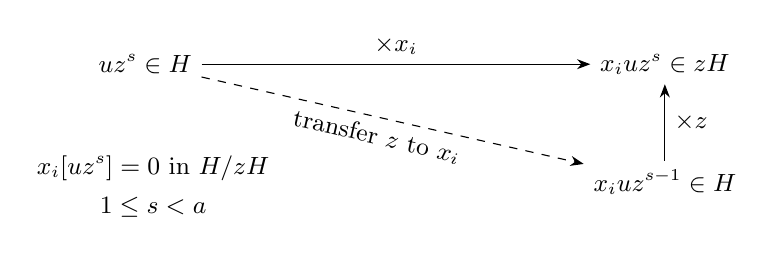
\begin{tikzpicture}[>=Stealth,font=\small]
\node (u) at (-3.3,0) {$uz^s\in H$};
\node (xu) at (3.3,0) {$x_iuz^s\in zH$};
\node (transfer) at (3.3,-1.5) {$x_iuz^{s-1}\in H$};
\draw[->] (u) -- node[above] {$\times x_i$} (xu);
\draw[->] (transfer) -- node[right] {$\times z$} (xu);
\draw[->,dashed] (u) --
  node[pos=.47,below,sloped] {transfer $z$ to $x_i$} (transfer);
\node[align=center] at (-3.2,-1.55)
  {$x_i[uz^s]=0$ in $H/zH$\\[3pt]
   $1\le s<a$};
\end{tikzpicture}
\caption{A middle slice is annihilated by every earlier variable.
The dashed arrow is supplied by box stability, or by an earlier
prescribed power if the monomial leaves the earlier-variable box.
Consequently all Koszul differentials on a middle slice vanish.
At $s=0$ there is no factor of $z$ to transfer; at $s=a$ the
last exponent is outside the box. These are the two endpoints.}
\label{fig:endpoint-slices}
\end{figure}


It remains to compare the two endpoint contributions.  Write
$\Lambda'$ for lex replacement with the earlier prescribed powers
in $R$.  The induction hypothesis applies to both $H^{(0)}$ and
$H^{(a-1)}$.  It gives an ideal comparison for the first and a
quotient comparison for the second.  Their respective lex
replacements have the same Hilbert functions, and hence the same
Koszul term dimensions.  Subtracting the Betti inequalities from
these dimensions gives
\begin{align}
 D^R_{p,j}(H^{(0)})
       &\ge D^R_{p,j}(\Lambda'H^{(0)}),
       \label{tor:induction-zero}\\
 D^R_{p,j-a}(R/H^{(a-1)})
       &\ge D^R_{p,j-a}(R/\Lambda'H^{(a-1)}).
       \label{tor:induction-top}
\end{align}
This also covers any coefficient ideal equal to $R$: its lex
replacement is $R$, the corresponding ideal comparison is equality,
and its quotient is zero.

The slice inequalities of Lemma~\ref{box:inequalities} imply
\begin{equation}
\label{tor:endpoint-inclusions}
 G^{(0)}\subseteq\Lambda'H^{(0)},\qquad
 \Lambda'H^{(a-1)}\subseteq G^{(a-1)}.
\end{equation}
Indeed, fix an earlier-variable degree $e\ge0$.  For the first
inclusion, apply the zero-slice inequality to the included exponent
sets of $H$ and $G$ in total degree $e$.  For the second, apply
the top-slice inequality in total degree $e+a-1$.  Each slice of
$G$ is already a lex segment in the earlier-variable box, so its
cardinality comparison with the corresponding slice of $H$ becomes
the stated containment in the appropriate lex replacement.
All monomials outside the earlier-variable box belong to both ideals.
This proves the inclusions in every degree.

Apply Lemma~\ref{tor:deficit} to the first inclusion in
\eqref{tor:endpoint-inclusions} and to the quotient map furnished
by the second:
\[
 R/\Lambda'H^{(a-1)}\longrightarrow R/G^{(a-1)}.
\]
Together with~\eqref{tor:induction-zero} and
\eqref{tor:induction-top}, this gives
\begin{align*}
 D^R_{p,j}(H^{(0)})&\ge D^R_{p,j}(G^{(0)}),\\
 D^R_{p,j-a}(R/H^{(a-1)})
       &\ge D^R_{p,j-a}(R/G^{(a-1)}).
\end{align*}
Adding and using~\eqref{tor:endpoint-deficits}, we obtain
\[
 D^R_{p,j}(B_H)\ge D^R_{p,j}(B_G).
\]
The equal Hilbert functions of $B_H$ and $B_G$ imply
\[
 \dim_\C K^R_p(B_H)_j
    =\binom{r-1}{p}\dim_\C(B_H)_{j-p}
    =\dim_\C K^R_p(B_G)_j,
\]
with the binomial coefficient interpreted as zero outside its range.
Subtracting the deficit inequality from these equal dimensions gives
$\beta^R_{p,j}(B_H)\le\beta^R_{p,j}(B_G)$.
Equation~\eqref{tor:reduction} proves the ideal comparison over $A$,
and~\eqref{tor:ideal-quotient} completes the quotient comparison.
Every step applies to every $p\ge0$ and $j\in\Z$; in particular,
negative internal degrees and Koszul terms outside their homological
range introduce no additional cases.
\end{proof}

\section{The prescribed lex-plus-powers ideal}\label{sec:assembly}

We now combine the comparisons, keeping the same ideal at every
homological and internal degree.

\begin{proof}[Proof of Theorem~\ref{thm:main}]
If \(I=S\), then \(L_d=S_d\) is allowed in every degree and \(J=S\);
all quotient Betti numbers are zero. Assume \(I\ne S\).
Proposition~\ref{mono:bound} gives a monomial ideal \(M\supseteq P\)
with the Hilbert function of \(I\) and
\[
 \beta^S_{p,j}(S/I)\le\beta^S_{p,j}(S/M)
 \qquad(p\ge0,\ j\in\Z).
\]
Proposition~\ref{stab:main} gives a box-stable monomial ideal
\(H\supseteq P\), with the same Hilbert function, and
\[
 \beta^S_{p,j}(S/M)\le\beta^S_{p,j}(S/H).
\]
By Proposition~\ref{box:ideal}, the degreewise box-lex replacement
\(G=\Lambda H\) is an ideal, with the same Hilbert function.
Theorem~\ref{tor:stable} gives
\[
 \beta^S_{p,j}(S/H)\le\beta^S_{p,j}(S/G).
\]

It remains to check that \(G\) is the ideal prescribed in
\eqref{eq:prescription}.
In degree \(d\), list all monomials in decreasing lex order and remove
those belonging to \(P_d\). The remaining list is exactly
\(\mathcal B_n(d)\) in decreasing lex order.
The monomials of \(G_d\) outside \(P_d\) are the first
\[
 q_d=\dim_\C I_d-\dim_\C P_d
\]
positions of this remaining list. This integer lies between zero and
\(|\mathcal B_n(d)|\), because \(H\supseteq P\) has the same Hilbert
function as \(I\).

Every box prefix is obtained by intersecting some full-list prefix with
the box. Thus a lex-segment subspace \(L_d\) with
\(\dim_\C(L_d+P_d)=\dim_\C I_d\) exists. Enlarging that full-list prefix
to the largest one of the same resulting dimension adds only monomials
already in \(P_d\), and does not change the sum. Consequently
\(L_d+P_d=G_d\) for every \(d\), including the empty and full box cases.
Hence \(J=G\). The displayed comparisons prove all the asserted Betti
bounds for this single \(J\).
\end{proof}

The argument proves idealness and all syzygy bounds together.
The use of \(\C\) enters the commuting-form construction and supplies the
roots of unity for stabilization; no conclusion in positive
characteristic is asserted for an arbitrary regular sequence.

\section{Arbitrary regular-sequence length and characteristic-zero fields}
\label{sec:characteristic-zero}

The new input of this paper is the Artinian theorem over \(\C\). We now
apply the published Artinian reduction and record the coefficient-field
argument needed for Corollary~\ref{cor:characteristic-zero}.

\begin{proof}[Proof of Corollary~\ref{cor:characteristic-zero}]
If \(I=S_F\), the prescription gives \(J=S_F\), and all quotient Betti
numbers vanish. We may therefore assume that \(I\) is proper.

First let \(F=\C\). After a linear change of coordinates, one may arrange
that
\[
 f_1,\ldots,f_c,x_{c+1},\ldots,x_n
\]
is a regular sequence; the list of variables is empty when \(c=n\).
Write \(\overline f_i\) for the images of the \(f_i\) in
\(\overline S=\C[x_1,\ldots,x_c]\). They form a full regular sequence
of degrees \(a_1,\ldots,a_c\). Theorem~\ref{thm:main}, applied in
\(\overline S\) to every homogeneous ideal containing this sequence,
gives both the Eisenbud--Green--Harris and lex-plus-powers assertions for
\(\overline f_1,\ldots,\overline f_c\).

The Artinian reduction of Caviglia--Maclagan
\cite[Proposition~10]{CM08} transfers the Hilbert-function assertion to
\(f_1,\ldots,f_c\). Theorem~4.1 of Caviglia--Kummini \cite{CK14}
transfers the Betti assertion as well. Their formulation uses Betti
numbers of ideals. For any proper homogeneous ideal \(K\) in a standard
graded polynomial ring \(A\), the exact sequence
\(0\to K\to A\to A/K\to0\) gives
\[
 \beta^A_{p+1,j}(A/K)=\beta^A_{p,j}(K)
 \qquad(p\ge0,\ j\in\Z).
\]
The remaining quotient Betti number is \(\beta^A_{0,0}(A/K)=1\).
Thus their convention is equivalent to the quotient convention used
here. The lexicographic embedding modulo \(P_F\) in that reduction
selects exactly the prescribed \(q_d\) greatest monomials outside \(P_F\)
in each degree. A linear change of coordinates preserves Hilbert functions
and graded Betti numbers, so this proves the corollary over \(\C\).

Now let \(F\) be any characteristic-zero field. Choose homogeneous
generators \(g_1,\ldots,g_r\) of \(I\), and let \(F_0\subseteq F\) be
the field generated over \(\Q\) by all coefficients of the \(g_i\) and
the \(f_i\). Set
\[
 S_0=F_0[x_1,\ldots,x_n],\qquad
 I_0=(g_1,\ldots,g_r,f_1,\ldots,f_c)\subseteq S_0.
\]
Then \(I_0S_F=I\). The sequence \(f_1,\ldots,f_c\) is regular in
\(S_0\): after tensoring each multiplication map with the faithfully
flat extension \(F/F_0\), it is the corresponding injective map over
\(S_F\). The finitely generated characteristic-zero field \(F_0\)
admits an embedding into \(\C\). Extending by this embedding preserves
regularity, so the case just proved applies to
\[
 S_{\C}=\C\otimes_{F_0}S_0,\qquad I_{\C}=I_0S_{\C}.
\]
No embedding of \(F\) into \(\C\) is needed.

Let \(J_{\C}\) be the resulting lex-plus-powers ideal. It is a monomial
ideal, so let \(J_0\subseteq S_0\) be generated by the same monomials and
put \(J_F=J_0S_F\). For \(E=F\) or \(E=\C\), let
\(S_E=E\otimes_{F_0}S_0\). Graded field base change preserves the
dimensions of homogeneous pieces. It also gives, for \(M_0=S_0/I_0\)
and for \(M_0=S_0/J_0\),
\[
 E\otimes_{F_0}\Tor^{S_0}_p(M_0,F_0)_j
 \;\cong\;
 \Tor^{S_E}_p(E\otimes_{F_0}M_0,E)_j.
\]
For example, this follows by tensoring the Koszul complex of the
variables with \(E\); its graded homology commutes with this flat
extension. Consequently the Hilbert equalities and Betti inequalities
over \(\C\) give the same equalities and inequalities over \(F\).
Finally, the monomials of \(P_F\) and the lexicographic order are
determined by their exponents, while the dimensions defining \(q_d\)
are unchanged by these field extensions. Hence \(J_F\) is precisely
the degreewise ideal \(J\) prescribed in the corollary.
\end{proof}

The argument changes the coefficient field only through extensions of
the common characteristic-zero field \(F_0\). It makes no assertion for
arbitrary regular sequences in positive characteristic.

\begin{thebibliography}{99}
\bibitem{Abedelfatah15}
A.~Abedelfatah,
\emph{On the Eisenbud--Green--Harris conjecture},
Proc. Amer. Math. Soc. \textbf{143} (2015), no.~1, 105--115.
\href{https://doi.org/10.1090/S0002-9939-2014-12216-7}{doi:10.1090/S0002-9939-2014-12216-7}.
Numbered statements refer to
\href{https://arxiv.org/abs/1212.2653v1}{arXiv:1212.2653v1}.

\bibitem{Bigatti}
A.~M.~Bigatti,
\emph{Upper bounds for the Betti numbers of a given Hilbert function},
Comm.\ Algebra \textbf{21} (1993), no.~7, 2317--2334.
\href{https://doi.org/10.1080/00927879308824679}{doi:10.1080/00927879308824679}.

\bibitem{BCR}
A.~M.~Bigatti, A.~Conca, and L.~Robbiano,
\emph{Generic initial ideals and distractions},
Comm.\ Algebra \textbf{33} (2005), no.~6, 1709--1732.
\href{https://doi.org/10.1081/AGB-200058217}{doi:10.1081/AGB-200058217}.
Author version:
\href{https://arxiv.org/abs/math/0308004}{arXiv:math/0308004}.

\bibitem{CDeS20}
G.~Caviglia and A.~De Stefani,
\emph{The Eisenbud--Green--Harris conjecture for fast-growing degree sequences},
Ann. Sc. Norm. Super. Pisa Cl. Sci. (5) \textbf{25} (2024), no.~3,
1753--1762.
\href{https://doi.org/10.2422/2036-2145.202203_025}{doi:10.2422/2036-2145.202203\_025}.
Numbered statements refer to
\href{https://arxiv.org/abs/2007.15467v2}{arXiv:2007.15467v2}.

\bibitem{CK14}
G.~Caviglia and M.~Kummini,
\emph{Poset embeddings of Hilbert functions and Betti numbers},
J. Algebra \textbf{410} (2014), 244--257.
\href{https://doi.org/10.1016/j.jalgebra.2014.04.007}{doi:10.1016/j.jalgebra.2014.04.007}.
Numbered statements refer to
\href{https://arxiv.org/abs/1210.5562v2}{arXiv:1210.5562v2}.

\bibitem{CM08}
G.~Caviglia and D.~Maclagan,
\emph{Some cases of the Eisenbud--Green--Harris conjecture},
Math. Res. Lett. \textbf{15} (2008), no.~3, 427--433.
\href{https://www.math.purdue.edu/~gcavigli/Articles-PDF/%5B4%5D.pdf}{Author manuscript}.

\bibitem{CS}
G.~Caviglia and A.~Sammartano,
\emph{On the Lex-plus-powers Conjecture},
Adv.\ Math.\ \textbf{340} (2018), 284--299.
\href{https://doi.org/10.1016/j.aim.2018.10.005}{doi:10.1016/j.aim.2018.10.005}.
Numbered statements refer to
\href{https://arxiv.org/abs/1802.03035v2}{arXiv:1802.03035v2}.

\bibitem{CL}
G.~F.~Clements and B.~Lindstr\"om,
\emph{A generalization of a combinatorial theorem of Macaulay},
J. Combin. Theory \textbf{7} (1969), no.~3, 230--238.
\href{https://doi.org/10.1016/S0021-9800(69)80016-5}{doi:10.1016/S0021-9800(69)80016-5}.

\bibitem{EGH}
D.~Eisenbud, M.~Green, and J.~Harris,
\emph{Higher Castelnuovo theory},
Ast\'erisque \textbf{218} (1993), 187--202.
\url{https://www.numdam.org/item/AST_1993__218__187_0/}.

\bibitem{FR}
C.~A.~Francisco and B.~P.~Richert,
\emph{Lex-plus-powers ideals},
in I.~Peeva (ed.), \emph{Syzygies and Hilbert Functions},
Lecture Notes in Pure and Applied Mathematics \textbf{254},
Chapman \& Hall/CRC, Boca Raton, FL, 2007, 113--144.
Author version:
\url{https://math.okstate.edu/people/chris/lpp-updated-final.pdf}.

\bibitem{Hulett}
H.~A.~Hulett,
\emph{Maximum Betti numbers of homogeneous ideals with a given Hilbert function},
Comm.\ Algebra \textbf{21} (1993), no.~7, 2335--2350.
\href{https://doi.org/10.1080/00927879308824680}{doi:10.1080/00927879308824680}.

\bibitem{Kuzmanovski}
N.~Kuzmanovski,
\emph{A Structural Property of Generic Initial Ideals},
preprint, 18 August 2026.
\href{https://arxiv.org/abs/2608.17281v1}{arXiv:2608.17281v1}.

\bibitem{MM}
J.~Mermin and S.~Murai,
\emph{The Lex-Plus-Powers Conjecture holds for pure powers},
Adv.\ Math.\ \textbf{226} (2011), no.~4, 3511--3539.
\href{https://doi.org/10.1016/j.aim.2010.08.022}{doi:10.1016/j.aim.2010.08.022}.
Author version: \url{https://s-murai.w.waseda.jp/papers/LPP.pdf}.

\bibitem{MPS}
J.~Mermin, I.~Peeva, and M.~Stillman,
\emph{Ideals containing the squares of the variables},
Adv.\ Math.\ \textbf{217} (2008), no.~5, 2206--2230.
\href{https://doi.org/10.1016/j.aim.2007.11.014}{doi:10.1016/j.aim.2007.11.014}.
Author version:
\url{https://pi.math.cornell.edu/~mermin/papers/ideals_containing_the_squares_of_the_variables.pdf}.

\bibitem{Murai}
S.~Murai,
\emph{Borel-plus-powers monomial ideals},
J. Pure Appl. Algebra \textbf{212} (2008), no.~6, 1321--1336.
\href{https://doi.org/10.1016/j.jpaa.2007.09.010}{doi:10.1016/j.jpaa.2007.09.010}.
Author version: \url{https://s-murai.w.waseda.jp/papers/BPP.pdf}.

\bibitem{ArtinianEGH}
OpenAI,
\emph{Commuting Division-Coefficient Forms and the Artinian
Eisenbud--Green--Harris Conjecture},
OpenAI Math Release preprint
\href{https://github.com/openai/math/blob/main/preprints/Commuting-Division-Coefficient-Forms-and-the-Artinian-Eisenbud-Green-Harris-Conjecture-September-23-2026/paper.pdf}{OAI:Commuting-Division-Coefficient-Forms-and-the-Artinian-Eisenbud-Green-Harris-Conjecture-September-23-2026},
2026.

\enlargethispage{2\baselineskip}
\bibitem{Pardue}
K.~Pardue,
\emph{Deformation classes of graded modules and maximal Betti numbers},
Illinois J. Math.\ \textbf{40} (1996), no.~4, 564--585.
\href{https://doi.org/10.1215/ijm/1255985937}{doi:10.1215/ijm/1255985937}.

\bibitem{Richert}
B.~P.~Richert,
\emph{A study of the lex plus powers conjecture},
J. Pure Appl. Algebra \textbf{186} (2004), no.~2, 169--183.
\href{https://doi.org/10.1016/S0022-4049(03)00130-0}{doi:10.1016/S0022-4049(03)00130-0}.
\end{thebibliography}

\end{document}
